% This file is based on the "sig-alternate.tex" V1.9 April 2009
% This file should be compiled with V2.4 of "sig-alternate.cls" April 2009

\documentclass[sts]{sig-alternate}
\usepackage[english]{babel}	
\usepackage{pdfpages}
\usepackage{graphicx}
\usepackage{amsmath}	
\usepackage[T1]{fontenc}

\usepackage{url}
\usepackage{etoolbox}

\makeatletter
\patchcmd{\maketitle}{\@copyrightspace}{}{}{}
\makeatother

%\crdata{0-00000-00-0/00/00}
\begin{document}

%%% Maketitle metadata
\newcommand{\horrule}[1]{\rule{\linewidth}{#1}} 	% Horizontal rule

\title{
		%\vspace{-1in} 	
		\usefont{OT1}{bch}{b}{n}
		\textbf{\normalfont\normalsize\textsc{Rochester Institute of Technology}} \\
		%\vspace{-10mm}		
		\horrule{0.5pt} \\[0.4cm]
		\textbf{\huge Big Data Medical Diagnosis} \\
		\horrule{2pt} \\[0.5cm]
		\vspace{-10mm}
}

\author{
		\normalfont\Large 
        Piter Garcia\\[0pt]\normalsize
        \today
}
\date{}
\maketitle


\section{Abstract}
	\label{Abstract}

	The use of the World Wide Web is continuously increasing and therefore it is an a useful tool, as a 		source of prediction purposes, for predicting a medical diagnosis based on an individual 					symptomatology. The topic I will be discussing is titled "Big Data Medical Diagnosis," in which I 		want to implement some models and strategies based on the papers cited below. I found the set of 			papers [1,2,3] and [4,5,6] interesting because it pertains to my topic of discussion which focuses 		on 	cleaning, web mining and prediction. The requirement for predicting the symptoms of users 			would be defined as the action to adapt information and services provided by a cleaned database to 		the need of a particular user. In the process, the database would be taking advantage of the 				knowledge gained from web browsing of the user.
	
	The ideology of strategies such as symptoms diagnosis, diagnosis popularity, and diagnosis 				performance were derived from the three last papers[4,5,6] I have chosen, and can be applied to 			medical databases. The development of each one of these strategies would 	allow us to build a hybrid 	system to better diagnose a medical problem and recommend a treatment protocol. There are multiple 		advantages that this hybrid system would have to offer in a medical database. First, predict a 			medical diagnosis of symptoms that currently afflict users. Second, give 	them recommendations for 		treatment based on their, or other users with similar problems, prior symptoms. Lastly, contribute 		to the implementation of a personalized system that would allow users to rank their diagnosis 			accordingly, as well as to diagnose other users with similar symptoms. 
	
	In order to develop this type of system, it is very important to implement a cleaning and 				preparation 	process of the data. Typically, the data recorded in medical databases is sparse and 			collected with no concerted effort to maintain data quality. For this process, I am using cleaning 		and preparation techniques such as Data Exploration, Data Discovery, and Data Quality. These 				techniques were obtained from the three first papers[1,2,3], which are very important for the 			cleaning process of a medical database. These research papers, the first three papers cited below, 		use different cleaning techniques to prepare the data, and to understand the overall process of 			knowledge discovery in a medical database environment.

\section{Introduction}
	\label{Introduction}

	My project is based on the analysis of six different research papers, which I have classified into 		Data Cleaning and Data Mining Analyses. The Data Cleaning Analysis is based on three 	papers that 			deal with "Exploration Mining in Diabetic Patients Databases," "Discovery of Temporal Patterns in 		Sparse Course-of-Disease Data," and "Data Quality in Genome Databases." The Data Mining Analysis is 		based on three papers that deal with "Predicting Content Change on the Web," "Predicting the 				Popularity of YouTube Videos," and "Predicting Performance." After a careful analysis of these 			papers I have taken their logical structure and modified them to meet the objectives of my project 		structure. The main purpose of my system is to predict users' diagnosis based on their symptoms. 			However, to better implement this system, I have separated the data cleaning and mining process. 			Furthermore, I incorporated the strategies of the three logical structures, in each analysis, 			mentioned above and 	coalesced them into a single logical structure. By employing this method, not 		only will it make the analysis of each paper's technique easier, it may also improve the accuracy of 	my system.\newline

	In order to maximize full use of the two obtained logical structure, I created a classification 			system which comprises of three categories for the two analyses. The first one is composed by the 		following; data exploration, data discovery, and data quality. The second one is composed by the 			following; symptoms diagnosis, diagnosis popularity, and diagnosis performance. By itself, each one 		of these categories provides a unique function. However, when linked together, they will improve the 	process of reaching a diagnosis for an individual.

	\begin{description}
  		\item\normalfont First Analysis \newline
  			In the first category of Data Exploration, derived from the first paper[1], the system would 			describe a semi-automatic means for cleaning a database of patients by exploring and 						understanding discovered rules. In the second category of Data Discovery, derived from the 				second paper[2], the system  would help understand the overall process of knowledge 						discovery in the medical database. In the third category, derived from the third paper[3], 				the system would compare error classes with existing solution  for data cleansing.
  					
  		\item\normalfont Second Analysis \newline
  			In the first category of Symptoms diagnosis, derived from the fourth papers[4]' technique, 				the 	system 	would predict a user's diagnosis by matching symptom description with those 					found in a database. In the second category of diagnosis popularity, derived from the fifth 				paper[5]' s 	technique, the system would allow users to know the diagnosis that have been 					predicted the most. This parameter would report to the system automatically and thus 						contribute to the improvement in accuracy of reaching a diagnosis. In the third category of 				diagnosis performance, derived from the sixth paper[6]' s technique, the system would allow 				users to provide feedback of whether or not the diagnosis and recommendation for treatment 				were accurate. This would help the system become smarter, and to keep a record of the user' 				s accurate diagnosis which would also contribute to an improvement in accuracy.		
	\end{description}
	
	Combining the above strategies, derived from the two sets of three papers in the first and second 		analysis, would allow us to build a more powerful and well-designed hybrid system to predict users' 		medical 	diagnosis accurately.

\section{Data Cleaning Analysis}
	\label{Data Cleaning Analysis}
	
	The Data Cleaning Analysis section is based on the analysis of the set of papers[1,2,3]. Each paper 		correspond to a category of this analysis, and it can be explained as follows: for the category Data 	Exploration, the analysis is based on the paper[1]. For the category Data Discovery, the analysis is 	based paper[2], and for the category Data Quality, the analysis is based on paper[3].
		
	\subsection{Data Exploration}
		\label{Data Exploration}
	
		This section is based on the paper[1] "Exploration Mining in Diabetic Patients Databases." In 			this paper[1] the authors came up with a semi-automatic data cleaning system to overcome the 				problem of noisy data. This system is based on a preliminary analysis of the database to reveal 			patient details such as their identification number, race, sex, date of birth, duration of 				diabetes, and date of screening. I could definitely use their approach to overcome noisy data 			within a medical database. However, in a system, such as the one I propose, the analysis would 			be mostly based on the duration user's symptom(s) and any test done.
	
		\begin{description}
  			\item[Semi-Automatic Data Cleaning:] \hfill \\
  				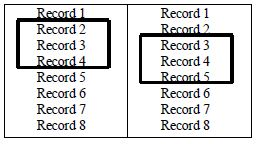
\includegraphics[scale=0.5]{cl1.eps} 
			
				This system is based on the "garbage in, garbage out" principle, and it is a crucial 						principle for data mining.  This approach allow users to define mapping between 							attributes in different format, and to decide whether or not the attributes are to be 					kept in the cleaned 	database to generate a standardize format. The analogy behind this 					is perfect to use on medical databases, especially for the system I propose, because 						medical data records are very inconsistent. On the other hand, this paper approach may 					cause duplicate records on a database. In order to fix this, using their suggested 						sorted neighborhood method would allow me to remove any duplicate record. They also use 					addition techniques, such as scrubbing data fields, to pre-process the data records 						before sorting them. In fact, these techniques could be used to remove typographical 						errors in a 	medical database without worrying about duplicate records.
  				
  			\item[Exploratory Mining Data:] \hfill \\
				This section is focused on the mining of classification and association patterns to 						provide 	description of the population having certain diabetic-related eye disease. They 				used this to predict whether or not a new patient is likely to have the eye disease. I 					noticed that with some modifications the same approach can be used to classify and 						associate user's symptoms to more accurately predict whether or not two users could have 				the same diagnosis. The 	algorithm they use to study how casual structures can be 							determined from association rules is LCD. This is a polynomial algorithm, which they use 				with dependence, independence, and conditional independence variables to restrict the 					possible causal relationship between variables.
  				
  				
\includegraphics[scale = 0.445]{cl2.eps} 
  				
  			\item[Markov Condition:] \hfill \\
				Let A be a node in a causal Bayesian network, and let B be any node that is not a 						descendant of A in the causal network. Then the Markov condition holds if A and B are 					independent 	conditioned on the parents of A.  
				
			\item[Dependence:] \hfill \\		
				The definitions of dependence and conditional independence are given as follows:
				
				\begin{itemize}
  					\item Dependence Test\newline 
  						Let s $\in$ (0,1) be a support threshold and c $\in$ (0,1) be a confidence 								threshold. An itemset S $\subseteq$ I is said to be (s,c) correlated if the 								following two conditions are met:
  						
  						\begin{enumerate}
 							\item The value of support (S) exceeds s;
  							\item The $X^2$ value for the set of items S exceeds the $X^2$  value at 									confidence level c.
  							
						\end{enumerate}

  					\item Independence test\newline
						Lets s $\in$ (0,1) be a support threshold and c $\in$ (0,1) be a confidence 								threshold. An itemset S $\subseteq$  I is said to be (s,c)-uncorrelated if 								the following two conditions are met:

  						\begin{enumerate}
 							\item The value support(S) exceeds s;
  							\item The $X^2$ value for the set of items S does not exceed the $X^2$ 									value at significance level c.
						\end{enumerate}
  					
  					\item Conditional Independence Test\newline
						variables $A$ and $B$ are independent conditioned on $C$ if p $(AB|C) = p(A|C) 							p(B|	C)$. The chi-squared test for conditional independence looks at the 									statistics $X^2(AB|C=0) + X^2(AB|C=1$), where $X^2(AB|C=i)$ is the chi-squared 							value for the pair $A$, $B$ limited to data where $C=i$. If $X^2(AB|C=0) + 								X^2(AB|C=1)$ is greater than the threshold value $X\propto^2$, the $A$ and $B$ 							are 	said to be dependent given condition $C$.
						
				\end{itemize}
		\end{description}

		Another implementation that would be of great use, when cleaning a medical database, is the 				new 	representation of the data used in this paper. The new representation is also known as 				general 	and exception rule representation. The reason why this would be a good implementation 			is because the general rules give the underlying trend in the data, and the exception rules 				give the abnormalities of those trends. This would make database more intuitive and draw 					more attention to the interesting patterns.

	\subsection{Data Discovery}
		\label{Data Discovery}
	
		This section is based on the paper[2] "Discovery of Temporal Patterns in Sparse Course-of-				Disease Data." This paper[2] focuses in discovering useful patterns in medical data to show 				group of patients having similar experiences during the course of a disease. Their approach is 			achieved by implementing a Temporal Pattern Discovery, better known as TEMPADIS. In a medical 			database, such as the one I propose, this approach would be ideal to discover users with similar 		patterns and facilitate a diagnosis prediction based on the similarity of their symptoms and 				other factors that may influence. \newline 

		\begin{description}
  			\item[Exploration and Preparation of a Medical Database] \hfill \\
				To find similar patterns they grouped users into categories according to specific 						reasons. In order to do this, they emphasize the importance of focusing on a subset of 					variables related to the knowledge to be discovered when implementing the KDD technique 					process.	\newline
			
				
\includegraphics[scale=0.37]{cl3.eps} 
			
  				\item[Data Cleaning and Selection] \hfill \\
					The main purpose of the cleaning and selection steps is to remove the noise from the 					data to develop strategies for coping with the data sparseness, and to find useful 						data features or invariant representations by reducing effective number of 								variables. Their strategy can help to find useful features to represent data based 						on the user's symptoms. This would allow any system to use only a minimum of key 							variable to well represent the data.
				
  				\item[Constructing and Merging the data-field] \hfill \\
 					To construct and merge the data filed, they use a single variable that represents 						the 	patient's general health status. Furthermore, they used a machine learning 							technique, a decision tree, to learn rules to determine a value used from a large 						dataset. As they mention, decisions trees are built using varying rules about the 						information gained by splitting the remaining unclassified examples on each of the 						remaining unused attributes. Therefore, for the project I propose, it is possible to						construct a set of data by randomly selecting x days from y patients to list all the 					symptoms experienced during 	x days. This would allow me to induce the tree to 							determine the correct medical diagnosis of one, or multiple patients, with the help 						of the C4.5 algorithm. The C4.5 is an algorithm, also used in this paper, that can 						convert the resulting tree into rules to determine medical diagnoses. Another method 					that they suggest, which could be added to the proposed system, is a severity 							measure. A severity measure would provide a way to differentiate between patients 						that have the same status with different diagnosis.	 	
 				
			\end{description}

	\subsection{Data Quality}
		\label{Data Quality}
	
		This paper is based on the paper[3] "Data Quality in Genome Databases." The main purpose of this 		paper[3] is the importance of drug discovery to create and maintain genome databases in 					commercial organizations. Medical databases are similar to genome databases in the sense that 			they both can have inaccurate, incomplete, outdated and in an overall poor state data. 					Therefore, using the methodology applied in this paper[3] may help to determine and improve data 		quality for medical databases. During their analysis they identified five classes from which 				only four could be of great use for poor medical data quality such as analysis errors, 					transformation errors, propagated errors, and state data.

		\begin{description}
  			\item[Errors in Data Production]  \hfill \\
  				\begin{enumerate}
  					\item Analysis errors - misinterpretation of information.
  					\item Transformation errors - bad transformations of information.
  					\item Propagated errors - erroneous data is used for the generation of new data.
  					\item Stale data - unnoticed changes to based data on which a data item depends and 						falsify 	it.	
				\end{enumerate}
  			
				They made use of two strategies to identify the producer errors. First, they developed 					detailed Information Product Maps (IP-Maps) for data production to provide them with a 					sound basis for quality improvement efforts. Second, for special cases of errors they 					use the 	Transitive Stale data, Annotation-Based Scale (TABS) standard, from the 							analysis of the data production process, to define classes of error such as false 						positive, over-prediction, domain error, false negative, under-prediction, undefined 						source, and typographical error. After a thorough analysis of these two strategies I 						have concluded that these two techniques are strictly for genome database and would not 					be very helpful with medical databases, such as the one I propose. However, using their 					ideology with a different approach may be useful to identify producer errors in medical 					databases, this requires further analysis.\newline

				The quality check is omitted on this paper because it is time consuming and expensive. 					This would not be the case for the system I propose due to its structure. The quality of 				the data and analysis could be check individually by allowing users to rate the outcome 					of the system. This could be a good way to start checking for the quality of the data 					and system improvement.
		  			
  			\item[Credibility checking and re-annotation]  \hfill \\			
 				In this section the authors, from the paper[3], propose a most reliable way for semantic 				error correction in 	their data, which is to re-perform experiments and computational 						analysis under careful control by domain experts. The idea they propose could be of 						great use in my system have different domain experts (algorithms) to collect arguments 					for correctness of the data, which could also be done through integrity constraint.	
  			
  			\item[Metadata management]  \hfill \\			
  				Learning how the information was gained, its interpretation, and the information this is 				based upon is one of the main problems in verifying the data correctness. In this paper 					the data lineage method is proposed to keep annotation up to date without having to re-					annotate when the data changes. Using data linage method in my system would allow data 					items that depend on changing data to be easily identified for re-analysis. In fact, the 				use of their general evidence functions for their domain analysis could enable me to 						build a model to specify my own cleansing process after implementing some changes to 						their structure. The intrinsic properties for the individual functions can be used to 					detect erroneous analysis in a medical databases if well implemented.
  			
		\end{description}
			
\section{Data Mining Analysis}
	\label{Data Mining Analysis}
	
	The Data Mining Analysis section is based on the analysis of the set of papers[4,5,6]. Each paper 		correspond to a category of this analysis, and it can be explained as follows: for the category Data 	Exploration, the analysis is based on the paper[1]. For the category Data Discovery, the analysis is 	based on paper[2], and for the category Data Quality, the analysis is based on paper[3].
	
	\subsection{Symptoms Prediction}
		\label{Symptoms Prediction}
	
		This section is based on the paper[4] "Predicting Content Change on the Web." Based on empirical 		analysis, I have found that utilizing user' s symptoms as well as other users' related symptoms 			diagnosis improves prediction accuracy. The development of this assumption is based 	on the web 		prediction approach. Here, they use numerous similarity metrics to identify related objects and 			focus specially on measures of temporal patterns similarity. This approach is suitable for 				symptoms prediction because, like web pages, symptoms diagnosis also tend to change with time. 			This approach looks for changes in the distribution of query that lead to a diagnosis, impacting 		the relevance of the current diagnosis to the query. Also, they use a personalized retrieval 				that provides an accurate prediction from revisiting a page with new contents. This means that 			by implementing such an approach in my proposed system, it may 	enable us to have a more 				accurate prediction by pushing new content to a user whose symptoms have been previously 					diagnosed.\newline

		The past observed values are considered as a prediction' s means basic. An example of 					this in 	my proposed system would be as follows. When predicting a diagnosis, we can simply 				predict 	based on the diagnosis observed over past historical window. However, this approach 				would not be very efficient on a user who has no record or whose symptoms are new. Therefore, 			having a medical database in which the user's symptoms can be mapped is trivial. In particular, 			as reference by this paper, the content of the object (symptoms) would provide us with a finer 			distinction of the degree of change that a particular diagnosis may be under-doing, and the 				relationship among other diagnosis within a database. Unlike their approach, in order for this 			system to have an efficient prediction it must use the reverse logic of this strategy. The 				reason for this is because, they are considering more significant objects that experience vastly 		dissimilar changes. This approach would not be efficient in our case because there would be an 			overwhelming amount of diagnoses that could not possibly be handled by the system, assuming we 			have a huge medical database; second, it would not provide the right diagnosis, assuming we have 		a small medical database. However, the reverse logic of this approach would give us a diagnosis 			with similar patterns.\newline

		In this paper[4], their web setting approach are based on natural choices of relationships types 		that include, distance of the object graph, similarity content, and similarity in temporal 				change pattern. This setting approach would be perfect for a medical diagnosis prediction system 		as the one I am proposing. In order for me to adopt such a model, I would need to implement the 			algorithm mentioned in this section of the paper, known as DTW algorithm. This algorithm is 				especially novel and it provides robust computation of similar temporal change patterns by 				dealing with the case where content between two objects(symptoms) may be correlated in time but 			slightly out of phase. Also, they develop an expert combination approach where the experts are 			selected according to the degree of relatedness and demonstrate the model choice superiority to 			other relational techniques. The expert combination approach, as expressed in this paper, would 			enable us to best incorporate related information sources into a machine learning algorithm. In 			addition, they incorporate features based on the content of the object as well as the content 			of other related objects. For this approach they present a novel algorithm to combine the 				information in an expert prediction 	framework, which examines techniques for identifying 				related objects including objects with similar content, and those with correlated content across 		time. The advantage of using this method is that it is broad-based and we could easily 					incorporate additional features. Also, their framework implementation would allow us to 					effectively  leverage information from related objects without the 	need for sampling from the 		current time slice.\newline
	
		The information sources of this paper[4] could be useful for the proposed medical diagnosis 				prediction system. This can be explained in three types of information settings. First, 1D 				setting where only user' s diagnosis information in previous time-stamps is used to estimate a 			diagnosis. Second, 2D setting where using a wider range diagnosis information about a user' s 			diagnosis would help us to estimate a future diagnosis. Third, 3D setting in which the diagnosis 		of the user can be compared to other diagnoses in order to determine the probability of a 				current or future diagnosis. This is one of their given scenarios, where information from a 				previous diagnosis is available and observed over a period of time to induce a function that can 		be used to estimate diagnosis based on changes in the user's symptoms.

		\begin{description}
  			\item[Framework Implementation:] \hfill \\				
  				The framework in this paper[4] could easily be implemented in my proposed system. If we 					let $O$ be a set of objects and $C \subseteq O$ be the goal concept. In our problem, $O$ 				is the set of symptoms and $C$ is the set diagnosis. In this paper, they applied a 						binary supervised learning setup that could be used in our framework as well. This is, 					$h(o) = 	1 <-> o \in C$ and let $E =$ \{$o_1$, $h(o_1)$, ..., $h(o_k)$\}, where $o_i$ 						$\in O$ and $h(oi) \in$ \{0,1\}, be a set of training examples. According to their 						implementation, we could extend this setup based on time in the following manner. Let $T 				=$ \{0, 1, ..., $\infty$\} be a discreet representation of time, where $h : OxT ->$ 						\{0,1\} is a temporal goal function and $E$ = \{$o_1$,$t_1$,$h(o_1,t_1)$,...,$o_k$,						$t_n$,$h(o_k,t_n)$\} is a set of temporal training examples where $o_i \in O, t_j \in T$ 				and $h(o_i,t_j) \in$ \{0,1\} Besides, this type of framework can use features of other 					objects. For example, they implement the function $f_i: O^k -> I_m(f_i$) that simulates 					a prediction determined on the content similarity of the predicted page $o$ with the 						other objects that are fed as input to produce $h(o,t)$. The diagnosis prediction, based 				on their based implementation, could be represented as following:

				\begin{enumerate}
  					\item Diagnosis(Symptoms(t)):\newline 
  						It means 1,equal to Symptoms(t) matched found.
  					\item Diagnosis(Symptoms(t)):\newline
  						It means 0,equal to Symptoms(t) matched not found.
				\end{enumerate}
			
				On the other hand, they intuitively assumed that the degree of content similarity and 					the 	similarity 	between content B, that changed, and A's full content may be 								indicative of the relationship strength. This means that accurate diagnosis from other 					users with similar symptoms may completely change a user' s diagnosis due to its 							relationship strength indicator.
		
  			\item[Algorithms] \hfill \\
 				This paper[4] used different type of algorithms based on their solution framework. Among 				these algorithms, the base line algorithm is found to be more suitable for my project 					implementation. This algorithm' s prediction is based on probability of users' symptoms 					and on the past training examples. In my case this training would be part of a medical 					database. This could be expressed as follows:\newline

				$P(h(o_i,t_i) = 1|(h(o_i,t_k) \in E$,\newline 
				where $t_k < t_j and (t_j-t_k)\leq1)$\newline
 				
  			\item[Algorithm Using Related Objects] \hfill \\	
  				They, authors in paper[4], use the related objects algorithm to collect information from 				other sources, such as a medical database in our case, into a single expert. This is 						used along with the use 	of multiple models to boost performance. This algorithm would 					be suitable for me to implement since it would consider multiple diagnoses features with 				those of the user.
  										
  			\item[Relational-Union and Stacking algorithm:] \hfill \\
				The RU algorithm was used in this paper[4] to extract an instant from the test and give 					this as 	an input to provide prediction. The way this was achieved was by using SVM 						classifier based on their objective, and creating scenarios relational features through 					the collection of features over related objects. Another algorithm explained in this 						paper is the bagging method. This, combined with majority voting, can be selected to use 				a trained model for each of the k-training sets. On the other hand, they applied a 						technique named graph KNN to identify the experts of an object by using in-link. Also, 					this same algorithm is used to find the closest neighbour by using an undirected 							representation of the links with a single step.\newline
				
				DTW would measure the similarity of two time series as a function of both time-lag and 					speed. For 	example, DTW will give high score to the similarity of symptoms in A and 						symptoms in B, even 	if A differs more than B, but they will have a similar patterns. 						DTW is a dynamic programming algorithm that tries to find an optimal match of the time 					series by stretching and compressing section of those time series. Another interesting 					technique that can be thought as a simple case of DTW is Cross-correlation. This is a 					measure of similarity to time series as a function for the time-lag that can be applied 					to the diagnosis prediction process. This analysis can be implemented in this system as 					shown below. Here, d = \{1...N is a \} possible delay, N is the minimal time series 						length, lambda is the time series variance, and E is the means of the corresponding 						series. The delay with the best correlation is chosen as the similarity.\newline
				
\includegraphics[scale = 0.5]{first.eps} 				
				  			
		\end{description}

		This paper[4] discusses several methods that reduce the size of every time series. This is done 			by dividing a method into frames where the time-series similarity algorithm can be performed 				later. This is one of the ways to efficiently identify similar series in a large database, and 			this is 	applied through the DTW algorithm. One additional concern presented in this project is 			that sorting snapshots is expensive because the scale prediction task is perform by multiple 				iterations. However, there is one method that can be used for the same purpose and this is 				cross-correlation. This method finds temporal experts with the best performance in our empirical 		study, such computation is on-line with no need to store the previous snapshot. In this paper[4] 		they prove that the more information they have, the more improves the prediction over the usage 			of objects. This implementation DTW would be useful in the development of my system. Here, they 			offer several ways of combining information from related objects, but would the most efficient 			one to find similarities in symptoms as object and predict based on prior information form the 			user itself or other users.\newline
	
	\subsection{Diagnosis Popularity}
		\label{Diagnosis Popularity}
	
		This section is based on the paper[5] titled "Using Early View Patterns to Predict the 					Popularity of YouTube Videos." This paper[5] presents two simple models to predict the future 			popularities of 	YouTube 	videos. Even though this topic may be completely different to my topic 			of interest, it still makes use of important models and techniques that support the design and 			evaluation of a wide range of systems. This could positively influence the accuracy and 					efficiency of a system, such as the one I proposed, because their application brings along an 			enormous and ever growing amount of users generated content. According to this paper, their 				implementation would bring support that would drive the design and management of various 					services in my system. In other words, managing those diagnosis that are more likely to happen 			first, in a certain period of time, would help my system to be more efficient since it would 				disregard a huge amount of data.	

		\begin{description}
  			\item[Performance:] \hfill \\
 		 		The performance applied in this paper could easily be implemented in my system. The 						reason why is because they only evaluate the performance of their prediction models, and					this could easily be done by just getting a simple binary feedback from the user 							identifying whether or not the diagnosis has been correct. This is how the performance 					criterion of my system would be based on this paper model.\newline

				
\includegraphics[scale = 0.5]{second.eps} 

				Therefore, for a collection C of multiple diagnosis, where C is one category for example 				flue. The mean RSE would be defined as follows: \newline

				In this paper[5] they only make use of the RSE implementation and not the mean RSE. This 				is because various services, for which popularity prediction is useful, relative errors 					tend to 	be more 	relevant and meaningful than absolute ones. However, in our case both 					implementation would be useful. This is because my system performance evaluation would 					be much simpler than the one elaborated in this paper since it is based on a simple set 					of Boolean values in each category.\newline

				
\includegraphics[scale = 0.5]{third.eps} 
  			
  			\item[Framework:] \hfill \\
				The models implemented in this paper are the S-H, ML, and MRBF model. One disadvantage 					of their method, which is not needed in my implementation, is that they require full 						information 	about users' votes in order to build user profiles. In our case, all we 						would need from the user is a confirmation based on whether the predicted diagnosis was 					corrected or not. This would allow my system to create a dataset of correct diagnosis 					that have been predicted more frequently than others. This would be the first dataset 					that my system would query to predict a diagnosis. 				
  				
  			\item[Szabo-Huberman (S-H) Model:] \hfill \\
 				I believe that this is a very important model in my system. The reason why is because in 				diagnosis, such as the flue and others, the system would be able, based on observation, 					to express the future popularity of this diagnosis. This feature would allow us to 						prevent 	epidemic and or diseases from spreading. Based on this paper's model we can 						implement the S-H model for the proposed system in the following manner:\newline

				\includegraphics[scale = 0.5]{four.eps} 

				In this case, parameters $(t_r); t_t$ is independent of the diagnosis v. Therefore, the 					future popularity of v is related to its early one by constant factor if $t_r and t_t$ 					are 	fixed Based 	on this 	paper S-H implementation, the optimal value for $(t_r) ,t_t$ 						with any given pair $(t_r; t_t)$ can be computed in a given training set C of diagnosis. 				Using their 	expression for $N_(v; t_r; t_t)$ from which 	they took its derivative and 					equated it to zero, the procedure would lead to the following expression:\newline

			\includegraphics[scale = 0.5]{five.eps} 

			\item[Multivariate Linear (ML) Model:] \hfill \\
				Another model used in this paper is the ML Model. According to their implementation the 					ML model is more powerful than the S-H model. The reason to this is because it allows 					assignment of different weights in each sampling interval.
			 				
  			\item[MRBF Model:] \hfill \\
				In this model they alter the prediction of a single parameter set ML model based on the 					similarity to certain videos. In their case, if a training set of videos compass the 						various 	popularity patterns, it indirectly incorporates information about the pattern 					of the video for which they predict the future popularity and adapt the prediction model 				to it. The technique they use to avoid this issue could also work to keep diagnosis with 				the same popularity from being in the same category. This technique is named Radial 						Basis Functions 	(RBFs). RBF is a real valued function whose 	value depends only on the 					distance between its inputs and the center as a given point. Based on their 								implementation, it is possible to create a Gaussian RBF with it as the center and 						capture its similarity with a target diagnosis in the following manner:\newline

				
\includegraphics[scale = 0.5]{six.eps} 

				In this case, lambda is the parameter and $X(v)$ is the ML model feature vector for the 					diagnosis v. From this, it is possible to compute the $RBF_vc$, as referenced in this 					paper, and use it as one of the features in the prediction model as shown below, where 					$C$ would be the set of training set examples chosen as centers and $W_vc$ is the model 					weight associated with the $RBF$ feature for $vc$ used for prediction purpose.\newline

				\includegraphics[scale = 0.5]{seven.eps} 
		\end{description}

		In this paper[5], they classify their dataset into Top and Random. I believe that only random 			or top dataset would not be as efficient for the proposed system. Having both datasets as 				part of my system may improve its efficiency by first querying the dataset that contains 					diagnosis with the highest popularity, and if this is not found then system would proceed to 				query the random data. This would avoid extensive search on diagnosis such as flue, 						allergies, among others, but it may take long for those diagnosis that have rarely been 					diagnosed in certain time period. Also, they removed many videos from their databases just 				because they were missing information. This may seem the model's implementation a bit less 				realistic for my system. However, due to the simplicity in which popularity of a 	diagnosis 				would be measure I believe it would give a result just as good or better 	as their implemented 			models.

	\subsection{Diagnosis Performance}
		\label{Diagnosis Performance}
	
		This section is based on the paper[6] "Predicting Performance." The paper used in this section 			is titled "Have You Done Anything Like That?: Predicting Performance 	Using Inter-category 				Reputation."This is the third paper and it is based on a 	reputation system that uses the average 		of past performance(s) across all transactions. This works by often adding a time-discounting 			mechanism or weighting feedback ratings by the size of the transaction. They explored how the 			past reputation of specific  tasks can be used to predict the future performance on other 				different tasks. Another approach that relates to their work is that based on on-line 					helpfulness reviews and community question answering. They also investigated various approach to 		predict review helpfulness that can exploit different sets of features.

		\begin{description}
  			\item[Framework:] \hfill \\
				They framework below are some of those that are covered in this paper[6] and that could 					highly help my system to improve in terms of accuracy and or efficiency. First, the use 					non-textual 	features such as click counts. This technique has been seen in platforms 						such as Yahoo! Answers, among others. Second, exploring community feedbacks to identify 					high quality content in CQA platforms. Third, extracting high quality answers, with only 				few labeled 	examples, through a developed semi-supervised coupled mutual reinforcement 					framework. Fourth, extracting high quality answers from the CQA platform by considering 					both quality and relevance. Finally, using trained classifier that select the highest 					quality answers.					
  			
  			\item[Algorithm:] \hfill \\
 				In this paper[6], they assume that the user had enough feedback ratings and had enough 					task completed in category j. Therefore, they use the user's prior performance to 						predict the 	performance for a new task in the same category. This feature at first may 					not seem as important as it is to a system such as the medical diagnosis prediction 						system. Nevertheless, this feature may turn my system into a more reliable and powerful 					system. The 	reason to this is because by monitoring the performance of users the system 				would be able to predict future performance on a medical perspective. In other words, 					the system would be able to predict users' future diagnosis and or complications due to 					the user prior and current medical or diagnose performance. To implement such algorithm, 				based on this paper, we can divide such algorithm into two different approach.\newline 

				First, the Binomial Approach, this is a very simple setting used to examine the case 						where user is performing diagnosis only within a category. In our case, this means only 					within one diagnosing group such as flue. Now, given a past history of n diagnosis 						within the given category, assuming the current quality is known $q_(i; j)$ of the user 					in category $j, x$ would be the expected diagnosis as "good" to follow a binomial 						distribution. Based on the approach implementation in this paper[6], using Bayesian 						statistics it may be possible to infer $q_(i; j)$ based on the number of good or bad 						diagnosis, an example of this is shown in figure 8.\newline 

				\includegraphics[scale = 0.5]{eight.eps} 

				Second, the Multinomial Approach is, according to this paper[6], used for more complex 					tasks. They, authors of paper[6], use this approach to extend previous model and account 				for a range of discreet outcomes to get a multinomial distribution of K possible 							outcomes, as shown in figure 9.\newline

				\includegraphics[scale = 0.5]{nine.eps}  

				I do not agree with the fact that they assume the binomial feedback is only used for 						small tasks. The reason why is because the difficulty of a task depends mostly on the 					algorithm in which you are applying such approach as well as its implementation. 	
				
  			\item[Point Estimate:] \hfill \\
  				In the binomial case the prior $\beta$($\propto$; $\beta$) or value of $q_(i,j)$ is:						\newline

				\includegraphics[scale = 0.5]{ten.eps} 

				In the multinomial model the prior D($\propto$), where $\propto$ = $\propto_1$,,							$\propto_(k)$,,$\propto_(K)$ the mean value of $q_(i,j)$ is:\newline

				\includegraphics[scale = 0.5]{eleven.eps} 
  				
		\end{description}
		
		In this paper[6] they use parameters to evaluate their models. One of the parameter $\theta \in 			(0,1)$ and it represents the threshold that separates good outcomes from bad outcomes. 					Above are two image representation of the estimated points based on the two approaches 					implemented in this chapter, the Binomial and Multinomial approach.
				
\section{Conclusion}
	\label{Conclusion}

	I was able to develop a theoretical implementation of my topic based on the summary of each one of 		the three papers selected for each analysis. The three papers, in each analysis, differ vastly in 		their approach and implementation strategy. However, the common denominator with the papers is that 		they all implement algorithms and techniques whose purpose is to clean the data and predict an 			output based on the behaviour of an input. After meticulous analysis of the strategies implemented 		in the papers, I realized that I could easily incorporate a similar model in my system, whose main 		objective is to clean and prepare a medical database to predict a diagnosis based on the symptoms of 	an user. Mapping each paper to one of my three main categories, in each analysis, proved useful 			because this helped to identify the importance of the logical structure of each paper so that it 			could be assigned to a substructure of the logical structure in the system I am proposing. The task 		being performed by the algorithm developed from each paper is unique and complementary to one 			another. The reason for this can be explained in the following manner. 
	
	In the first analysis, all three papers[1,2,3] share one goal in common that is to clean and 				prepare the 	data before any mining algorithm is implemented. They all implement techniques of data 		exploration, data discovery, and data quality, but with different level of efficiency. The goal of 		this paper was to pick a technique, best implemented by each paper, that can improve the cleaning 		process of a medical database. Afterwards, blend these three best techniques into a hybrid system 		that can help the medical database to explore and understand the process of knowledge discovery to 		the best of 	its usage. 
	
	In the second analysis, its development can be explained as following. In the forth paper[4]titled 		"Predicting Content Change on the Web," which can be thought of as the main substructure used to  		predict a user's diagnosis. However, if we were to implement this based on the strategy used in this 	paper, along with other techniques, the outcome would not be very efficient. 	The reason for this is 	because it would take too long to give an answer, assuming we are using a large medical database; 		this may also prove to be inaccurate. Also, it may not be diagnostic at all, 	assuming we are using 		a small dataset. On the other hand, if we incorporate the strategy of the fifth paper[5] titled, 			"Using Early View Patterns to Predict the Popularity of YouTube Videos," we would be incorporating a 	very useful technique which would enable the system to have two classified datasets in which most 		diagnoses with the highest popularity would be queried first, followed by those that are not. This 		would speed up the system and make it run in a more efficient manner. Also, it would allow the 			system to personalize the data and classify it in a well organized way through user feedback. 			Furthermore, if I incorporated to my system the strategies obtained from the sixth paper[6] titled 		"Have You Done Anything Like That? Predicting Performance Using Inter-category Reputation,"we would 		be reinforcing not only the feedback given by the user to the system, but also incorporating a 			strategy that would provide users with recommendations and feedback based on the system's medical 		performance. 
	
	This hybrid system would be advantageous for the user, as well as institutions and 	society at 			large, in order to prevent and avoid epidemics or any diseases from spreading. Although none of 			the three papers had anything in common based on their titles, from an algorithm 	perspective all 			shared the same goal of prediction. This goal is what I based my analysis on in order to make use of 	the strategies and techniques outlined in the papers. There were instances in which I did not agree 		with the implementation and techniques in the three papers because it was not pertinent to the 			logical structure of my system. Examples of these include the Multinomial approach and the Random 		Sampling that were implemented in the third paper and strategies such as ML and MRBF are not really 		necessary for implementation in my system. I found that all papers contained adequate and important 		information that could be potentially useful to clean, prepare, and implement the Big Data Medical 		Diagnosis System.

\section{Reference}
	\label{Reference}

	[1] Wynne Hsu, Mong Li Lee, Bing Liu, Tok Wang Ling: Exploration Mining in Diabetic Patients 				Databases: Findings and Conclusions." School of Computing National University of Singapore 1-7.			\newline
	
	[2] Jorge C. G. Ramirez1,2, Lynn L. Peterson1, Diane J. Cook1, Dolores M. Peterson2: Discovery of 		Temporal Patterns in Sparse Course-of-Disease Data." Department of Computer Science and Engineering 		University of Texas at Arlington 1-23.\newline

	[3] Heiko M~ Aijller, Felix Naumann, Johann-Christoph Freytag: DATA QUALITY IN GENOME DATABASES." 		Humboldt University Berlin, Germany 1-16.\newline

	[4] Kira Radinsky, Paul N. Bennett: "Predicting content change on the web." 415-424.\newline
	
	[5] Henrique Pinto, Jussara M. Almeida, and Marcos Andre Goncalves: Using early view patterns to 			predict the popularity of youtube videos." 365-374.\newline	

	[6] Marios Kokkodis, Panagiotis G. Ipeirotis: Have you done anything like that?: predicting 				performance using intercategory reputation." 435-444.\newline
	
	\bibliographystyle{abbrv}
	\bibliography{report}
\end{document}